\section{Auswertung}
\label{sec:Auswertung}
\subsection{Theoretische Berechnung}
Zur Berechnung der Suszeptibilität der verschiedenen Materialien werden die Hund'schen Regeln (\ref{}) verwendet. Die sich ergebenden Werte für $L$, $S$ und $J$ 
sind in Tabelle (\ref{tab:L_S_J}) zu sehen. Die Größe $N$ wird mithilfe von 
\begin{equation}
  N = 2 \cdot \frac{\rho_w N_a}{M}
\end{equation}
berechnet. $N_a$ steht dabei für die Avogadrokonstante, $M$ für die Molare Masse und $\rho_w$ für die Dichte der Probe.
Die probenspeziefischen Werte sind in Tabelle (\ref{tab:L_S_J}) aufgelistet.

\begin{table}[H]
  \centering
  \caption{Theoriewerte für $L, S$, $J$ und $g_J$}
  \label{tab:L_S_J}
  \begin{tblr}{colspec={c c c c c c c c}}
      \toprule
      $\text{Material}$ & $L$ & $S$ & $J$ & $g_J$ & $\cdot \, 10³ \, \rho_w \,\left[ \unit[per-mode=fraction]{\kilo\gram\per\cubic\meter} \right]$ & $\cdot \, 10^{-3} \, M \, \left[ \unit[per-mode=fraction]{\kilo\gram\per\mol} \right]$ & $\cdot \, 10^{28} \, N \left[\frac{1}{\unit{\cubic\meter}}\right]$ \\
      \midrule
      \text{Nd} & 6 & 1,5 & 4,5 & 0,7272 & 7,24 & 336,5 & 2,59 \\
      \text{Gd} & 0 & 3,5 & 3,5 & 2,0000 & 7,40 & 362,5 & 2,46 \\
      \text{Dy} & 5 & 2,5 & 7,5 & 1,3333 & 7,8 & 373,0 & 2,52 \\  
      \bottomrule
  \end{tblr}
\end{table}

Die mithilfe von Formel (\ref{}) berechnete Suszeptibilität in Tabelle (\ref{tab:chi_theo}) aufgelistet. 
\begin{table}[H]
  \centering
  \caption{Theoriewerte für $\chi_{\text{theo}}$}
  \label{tab:chi_theo}
  \begin{tblr}{colspec={c r}}
      \toprule
      $\text{Material}$ & $\cdot \, 10^{-3} \, \chi_{\text{theo}}$ \\
      \midrule
      \text{Nd} &  2,9877\\
      \text{Gd} &  13,6565\\
      \text{Dy} &  25,0409\\  
      \bottomrule
  \end{tblr}
\end{table}

\begin{figure}
  \centering
  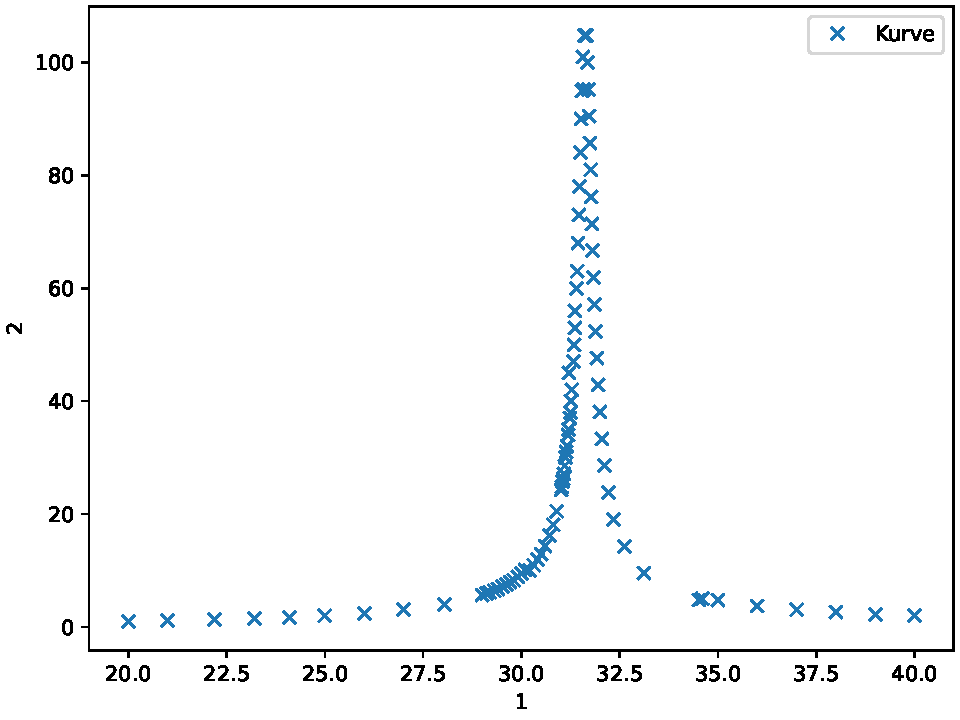
\includegraphics{plot.pdf}
  \caption{Plot.}
  \label{fig:plot}
\end{figure}

%Siehe \autoref{fig:plot}!